\section{Related Work}
\vspace{-5pt}


\noindent \textbf{Self-Alignment.}
Traditional alignment approaches rely heavily on extensive human-annotated preference data and complex reward model training through reinforcement learning, which poses significant scalability and cost challenges~\cite{ouyang2022training}. Self-alignment focuses on aligning LLMs themselves with model-generated feedback, datasets, critique, etc., which are then used for fine-tuning or training reward models~\cite{lee2023rlaif, bai2022training, cao2024towards, wang2024step, guo2024human}. Notable examples include synthesizing alignment training data with human-provided instructions and ICL examples~\cite{wang2022self, kim2023aligning, sun2024principle}, augmented web documents~\cite{li2023self}, or self-critique~\cite{bai2022constitutional, madaan2024self}. However, most of these methods still require an SFT/RLHF-tuning process to enhance alignment, along with some degree of human annotations or supervision. In contrast, \ours shares similar self-alignment principles using self-critique error feedback to gradually align the model, but it achieves this entirely without any model tuning or human supervision.



\begin{figure*}[ht]
    \centering
    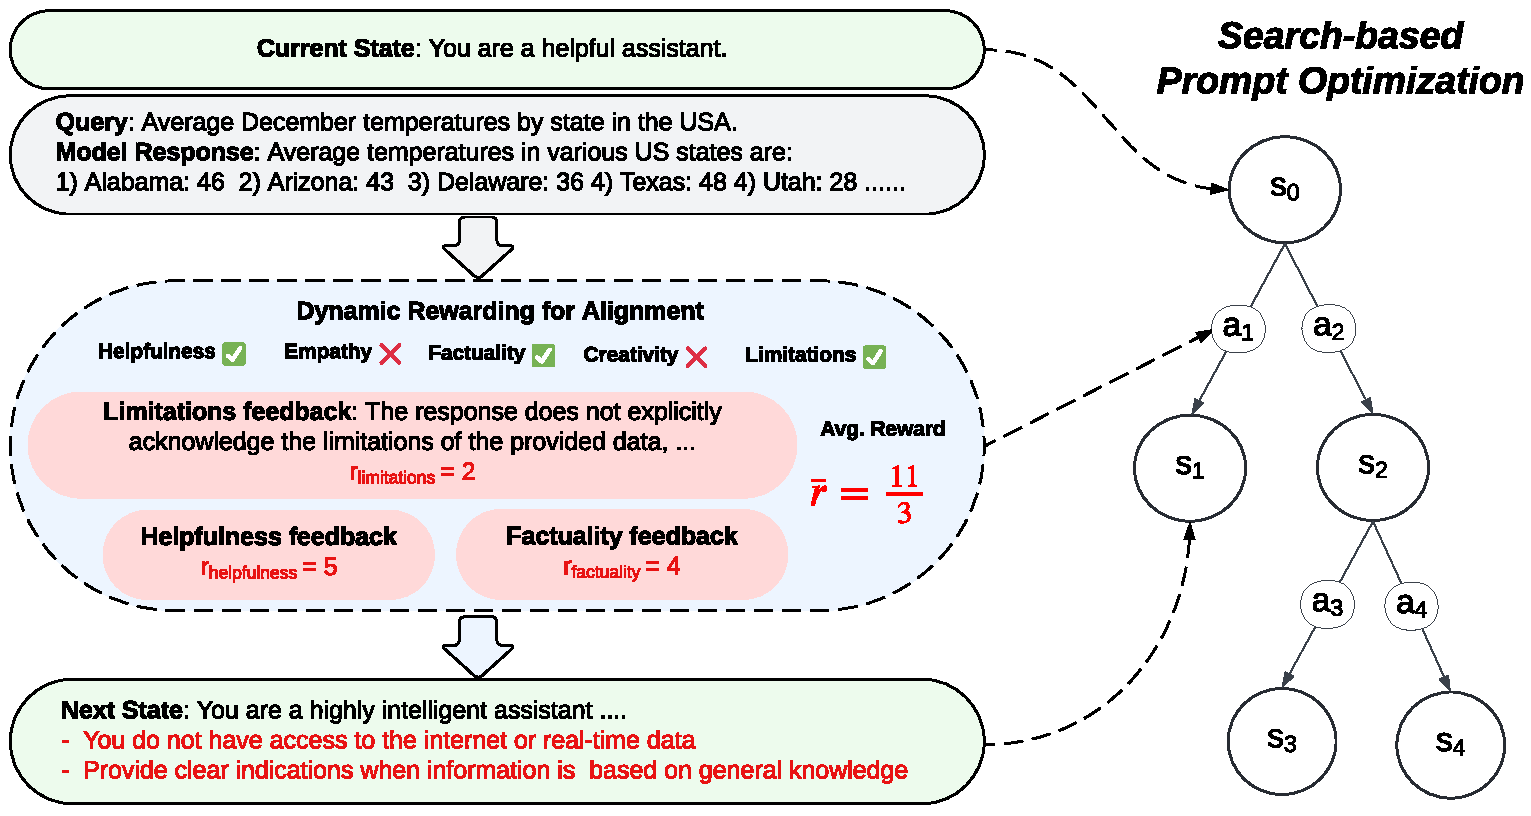
\includegraphics[width=0.95\linewidth]{images/Dynamic_Rewarding.pdf}
    \vspace{-8pt}
    \caption{Overall framework of Dynamic Rewarding with Prompt Optimization (\ours). The optimization problem is modeled as a Markov Decision Process (MDP) and solved using beam search to optimize the alignment prompt. Dynamic rewarding, a novel technique integrated into this framework, allows flexible reward assignment to detect and address alignment weaknesses in the current LLM, thereby enhancing the overall optimization process.
    }
    \label{fig:dynamic_rewarding}
    \vspace{-15pt}
\end{figure*}




\noindent \textbf{Tuning-Free Alignment.}
A recent trend in alignment research is to align LLMs without updating their parameters, typically as a post-training process for LLMs. This has witnessed two major lines of work recently. The first aligns models with carefully curated human annotations and ICL examples~\cite{han2023context, Lin2024ReAlign, zhao2024context}, while the second involves decoding-based methods to guide token generation and search with alignment rewards~\cite{li2023rain, khanov2024args, huang2024deal}. Although tuning-free, the first approach still requires human curation and often underperforms compared to SFT/RLHF-tuned counterparts. The second one, while effective, incurs higher inference costs per query, making it computationally expensive. It is worth mentioning that another recent promising direction is cost-efficient alignment through representation engineering~\cite{zou2023representation, wu2024reft}, which aims to steer LLM representation vectors for alignment~\cite{li2024inference, kong2024aligning, wang2024inferaligner}. However, these methods are not fully tuning-free and typically require additional data or model training to identify alignment directions in the embedding space. Nevertheless, \ours requires no additional annotations or model training, and also only needs a one-time optimization per model to achieve better performance than SFT/RLHF-tuned counterparts. 







\noindent \textbf{Prompt Optimization.}
Discovering optimal discrete prompts becomes far more crucial nowadays. Modern prompts for LLMs can be generally divided into two parts: in-context learning examples and detailed instructions. The former is usually treated as a retrieval problem with various schemas to select the influential examples~\cite{rubin2021learning, dong2022survey}. Optimizing the latter has been heavily studied recently, mostly formulated as a sampling or search problem. Generally, an initial prompt (e.g., a base prompt, ``You are a helpful assistant'') is given to start an iterative process, where diverse prompt candidates are generated per turn, and the best ones are kept for the next iteration. Various sampling strategies are proposed to diversify the prompt candidates, e.g., back translation~\cite{xu2022gps}, evolutionary operations~\cite{fernando2023promptbreeder}, self-critique~\cite{wang2023promptagent}. Different search frameworks also have been studied, such as Monte Carlo search~\cite{zhou2022large}, evolutionary algorithms~\cite{fernando2023promptbreeder, yang2023large}, beam search~\cite{pryzant2023automatic}, and Monte Carlo tree search (MCTS)~\cite{wang2023promptagent}. \ours builds upon recent search-based optimization methods but introduces novel techniques, such as dynamic rewarding, to effectively address the alignment problem. 